% ===========Für anderes Kapitel eventuell verwenden
% Für die Anzeige der Wortuhr werden adressierbare RGB-Leuchtdioden (LEDs) vom Typ WS2812B eingesetzt. 
% Diese ermöglichen eine individuelle Ansteuerung 
% jeder einzelnen LED innerhalb eines Verbunds. Die LEDs sind dabei physikalisch in Reihe 
% geschaltet (Daisy-Chain) und werden über eine einzige serielle Datenleitung gesteuert. 
% Jede LED verfügt über einen integrierten Controller, der die eingehenden Datenpakete 
% verarbeitet, den für sich bestimmten Anteil extrahiert und das verbleibende Signal für 
% die nachfolgenden LEDs aufbereitet und weiterleitet~\cite{Worldsemi2013}. 

\section{WS2812B LEDs als Anzeigeelement}
Die WS2812B ist eine integrierte RGB-Leuchtdiode mit eingebauter Steuerelektronik. 
Sie kombiniert eine Lichtquelle und eine digitale Ansteuerlogik in einem gemeinsamen Gehäuse der Bauform 5050. 
Dadurch entfällt die Notwendigkeit externer Treiberschaltungen für einzelne LEDs, was den Schaltungsaufwand reduziert und die Integration vereinfacht~\cite{Worldsemi2013}.

Ein wesentliches Merkmal der WS2812B ist die serielle Ansteuerung über eine einzelne Datenleitung. 
Die Kommunikation erfolgt über ein digitales Protokoll, bei dem die Daten bitweise übertragen werden. 
Jede LED empfängt dabei einen Datenstrom, verarbeitet die ersten 24 Bit zur eigenen Darstellung und leitet die verbleibenden Daten an nachfolgende LEDs weiter. 
Dieses Prinzip ermöglicht die Realisierung langer LED-Ketten mit minimalem Verdrahtungsaufwand~\cite{Worldsemi2013}. 

Die Farbdarstellung basiert auf drei integrierten Leuchtdioden für die Grundfarben Rot, Grün und Blau. 
Für jede dieser Komponenten stehen 8 Bit zur Verfügung, wodurch sich insgesamt 24 Bit pro LED ergeben. 
Dies ermöglicht die Darstellung von bis zu 16.777.216 verschiedenen Farbwerten. 
Die Datenübertragung erfolgt in einer fest definierten Reihenfolge der Farbkanäle, wodurch eine konsistente Farbwiedergabe gewährleistet wird.
Die Versorgung der WS2812B erfolgt mit +5V. 
Jede LED enthält eine interne Konstantstromsteuerung, wodurch eine gleichmäßige Helligkeit unabhängig von Versorgungsschwankungen erreicht wird~\cite{Worldsemi2013}. 

Ein weiterer Vorteil liegt in der Möglichkeit zur einfachen Kaskadierung (vgl. Abb.~\ref{fig:KaskadeLED}).
Mehrere LEDs können direkt hintereinander geschaltet werden, wobei der Ausgang einer LED mit dem Eingang der nächsten verbunden wird. 
Die maximale Anzahl der kaskadierbaren LEDs hängt primär von der Datenrate und der gewünschten Aktualisierungsfrequenz ab. 
Bei typischen Anwendungen können mehrere hundert bis über 1000 LEDs ohne zusätzliche Signalverstärkung betrieben werden~\cite{Worldsemi2013}.

\begin{figure}[H]
	\centering
	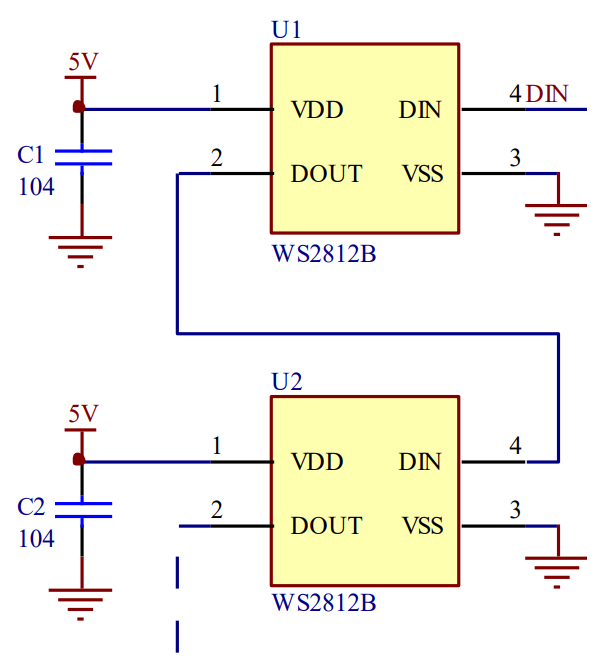
\includegraphics[width=0.5\linewidth]{inhalt/bilder/KaskadeLED.png}
	\caption{Schaltbild zur Kaskadierung von WS2812B LEDs mit einer Versorgungsspannung von +5V. Mit VDD als Versorgungsspannung, DIN als Datensignal Eingang, DOUT als Datensignal Ausgang und VSS als als Ground~\cite{Worldsemi2013}.}
	\label{fig:KaskadeLED}
\end{figure}

Für Anwendungen wie Wortuhren ergibt sich aus diesen Eigenschaften eine geeignete Architektur. 
Die einzelne Adressierbarkeit ermöglicht die gezielte Darstellung wobei die geringe Anzahl benötigter Steuerleitungen in einem geringen Verdrahtungsaufwand resultiert. 
Gleichzeitig erlaubt die hohe Farbauflösung eine flexible Gestaltung der Anzeige, beispielsweise zur Differenzierung von Funktionen oder Zuständen~\cite{Worldsemi2013}.

% LED-Typen (RGB, adressierbar)
% Ansteuerungsprinzipien
% Vor- und Nachteile
% RGB-LEDs
% Adressierbare LEDs (z. B. WS2812, SK6812)
% LED-Matrix
% LED-Streifen
% PWM-Helligkeitssteuerung
% Farbtemperatur
% Gleichmäßige Ausleuchtung
% Diffusoren (Acryl, Milchglas)
% Lichtkammern / Trennstege
% Hot-Spot-Vermeidung
% Energieeffizienz von LEDs

% adressierbare RGB-LEDs, NeoPixel/WS2812-Prinzip, Datenleitung, RGB-Farbmischung, Helligkeitssteuerung, LED-Matrix, separater Sekundenring
% adressierbare LEDs (WS2812 / NeoPixel)
% serielle Datenübertragung (1-Draht-Protokoll)
% RGB-Farbmodell (additive Farbmischung)
% Helligkeitssteuerung (PWM / softwareseitige Skalierung)
% Verkettung mehrerer LEDs (Daisy Chain)
% Timing-Anforderungen
% Energiebedarf pro LED
% Matrix vs. Streifen
% separater Sekundenring als Zusatzanzeige